\documentclass[a4paper,12pt]{article}

\usepackage{graphicx}
\graphicspath{ {./imgs/} }
\usepackage{fullpage}
\usepackage{amsmath}
\usepackage[ruled,vlined]{algorithm2e}
\usepackage{multicol}

\usepackage{geometry}
 \geometry{
 a4paper,
 total={170mm,257mm},
 left=10mm,
 right=10mm,
 top=2mm,
 bottom=2mm,
}

\setlength{\columnsep}{10mm}

\begin{document}

\title{\Large{\textbf{50.001 2D Submission \\ Group No. 30 }}}
\author{Daniel Low Yu Hian (1004372); \\ 
Sim Jia Ren (1004401); \\ 
Sean Gunawan (1004414); \\ 
Chan Jun Hern, Cawin (1004487); \\ 
Huang He (1004561)}

\maketitle

\begin{multicols}{2}

\subsection*{Solver algorithm}

\textbf{Step 0}: Check if the list of clauses is empty, if yes, returns the env mapping.\\
\\
\textbf{Step 1}: Traverse through the list of clauses,
trying to find a unit clause (that only contains one literal). 
In the meanwhile, keep track of the minimum size of clause 
(that contains the least number of literals). \\
\\
If a unit clause is found, set the literal to True or False such that this clause is True, 
call $substitute()$ to simplify the clauses, then, recursively call the solver with the new env mapping.
Solver returns the env mapping if a solution is found and returns $null$ if no solution is found.\\
\\ 
The solver will proceed to Step 2 if no unit clause is found. 
But by now we have got the $smallestClauseSize$ as an integer. \\
\\
\textbf{Step 2}: We can get a clause that satisfy $clause.size() == smallestClauseSize$
by traverse through the list of clauses for the second time. 
We break out of the traversal loop once we find the first one that satisfies, 
it helps reduces some unnecessary running time.\\
\\
\textbf{Step 3}: Once we have picked one of the shortest clause, 
we simply pick the first literal from that clause, set the positive literal to True,
call $substitute()$ to simplify the clauses, then, 
recursively call the solver with the new env mapping.\\
\\
if the returned env is $null$, which signifies no solution, we get the negative literal
and set it to False, call $substitute()$ to simplify the clauses, then, 
recursively call the solver with the new env mapping.\\
\\
\textbf{In summary}, the algorithm will try find a solution from setting unit clause to True. 
If there is no unit clause, it starts trying from the shortest clause first, until reaching the last clause.
Whenever a solution is found, the program will return the env that contains the satisfiable solution.
If no solution is found, the program will return $null$.

\subsection*{Substitute algorithm}

The simplification of clause list is done by $substitute()$, it is given a clause list 
and a literal, returns a new clause list after simplification assuming the literal is True.
It simply traverse through the clause list, call the $reduce$ function 
if the literal variable is present in the clause.

\subsection*{Test Result on test\_2020}
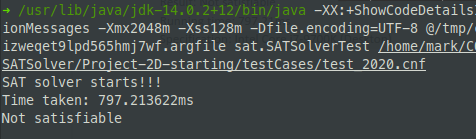
\includegraphics[width=0.5\textwidth]{result.png}
\textbf{Result}: Not Satisfiable \\
\textbf{Running Time}: 797.21 ms \\
\textbf{Machine Specs}: Intel Core i7-9700K (Desktop) (System: Ubuntu 18.04) (JDK: 14.0.2)\\

\end{multicols}


\end{document}